\documentclass[a4paper,12pt,twoside]{report}
\usepackage[left=2cm,right=2cm,top=2cm,bottom=3cm]{geometry}


\usepackage[utf8]{inputenc}
\usepackage{amsmath}
\usepackage[spanish, es-tabla]{babel}
\usepackage{amsfonts}
\usepackage{amssymb}
\usepackage{multirow, array} 
\usepackage{chngcntr}
\usepackage{graphicx}
\usepackage{subfig}
\usepackage{cite}
\usepackage{adjustbox}
\usepackage[table]{xcolor}


\usepackage{color}   %May be necessary if you want to color links
\usepackage{hyperref}
\hypersetup{
    colorlinks=true, %set true if you want colored links
    linktoc=page,     %set to all if you want both sections and subsections linked
    linkcolor=blue,  %choose some color if you want links to stand out
}

\title{}
\begin{document}
\begin{center}
\thispagestyle{empty}
\fontsize{12pt}{12pt}\selectfont 

%%%%%%%%%%%%%%%%%%% PORTADA %%%%%%%%%%%%%%%%%%%%%%%%


\textbf {\huge Diseño y calibración de un telescopio de muones híbrido para estudios vulcanológicos.}


\vspace{3cm}

{\large \textbf{Autor:}}

\vspace{0.5cm}

\large Jesús Peña Rodríguez

\vspace{3cm}
{\large \textbf{Director}}\\
\vspace{0.5cm}
{\large Luis A. Núñez}\\
\vspace{0.5cm}
{\large \textbf{Codirector}}\\
\vspace{0.5cm}
{\large Hernán Asorey}
\vspace{3cm}


\normalsize
\large Presentado como requisito del programa de 
\linebreak
\large Doctorado en Ciencias Naturales - Física

\vspace{4cm}

\large Universidad Industrial de Santander\\

\large  Facultad de Ciencias \\

\large  Escuela de Física - Abril 2019
    
  \end{center}
\large


\newpage
%%%%%%%%%% CONTENIDO %%%%%%%

\tableofcontents % indice de contenidos

\cleardoublepage
\addcontentsline{toc}{chapter}{Lista de figuras} % para que aparezca en el indice de contenidos
\listoffigures % indice de figuras


\chapter{Planteamiento del problema}

La muongrafía es una técnica no-invasiva que se utiliza para estudiar grandes estructuras antrópicas o naturales. Sus aplicaciones van desde detección de materiales ocultos en contenedores \cite{Blanpied2015}, arqueología \cite{Morishima2017, Gmez2016, Alvarez1970}, exploración geológica en Marte \cite{Kedar2013}, inspección de plantas nucleares \cite{Fujii2013}, cavidades subterráneas \cite{Saracino2017} y  vulcanología \cite{Tanaka2005, Tanaka2009, Lesparre2010, Lesparre2011, Lesparre2012}.\\

Actualmente las herramientas más utilizadas en el estudio de volcanes son la sismología, gravimetría y tomografía eléctrica. Estas tienen una resolución espacial y capacidad de penetración baja \cite{RosasCarbajal2017}, además los datos deben ser registrados de manera directa sobre la superficie del volcán, \cite{Marteau2012}. La muongrafía ofrece una alternativa con resolución espacial de decenas de metros \cite{Lesparre2012}, una gran capacidad de penetración y la adquisición de información es no-invasiva \cite{Nishiyama2014}.\\

Su funcionamiento se basa en la medición del flujo de muones que cruzan la estructura en diferentes direcciones. Esta medición se hace a través de un hodoscopio\footnote{Instrumento que mide la trayectoria de partículas cargadas haciendo uso de dos o más planos de detección}. Las diferencias de flujo que se proyectan sobre el elemento sensible permiten extraer información de la densidad interna del objeto escaneado.\\

Sin embargo, esta metodología presenta algunos problemas como la sub-estimación de la densidad debido al registro de eventos falso-positivos, los cuales se generan por tres fuentes: los muones horizontales que inciden desde la parte trasera del detector, los muones de baja energía que son dispersados por la superficie del volcán y partículas cargadas procedentes de lluvias aéreas extendidas (EAS) \cite{Nishiyama2014,Gomez2017}.\\

Para reducir estos efectos se han desarrollado diversas técnicas basadas en: la implementación de sistemas de medición del tiempo de vuelo (ToF) para eliminar los muones de albedo\footnote{Muones atmosféricos reflejados hacia la atmósfera por la tierra o generados en ella.)} \cite{Marteau2014, Cimmino2017}, la instalación de paneles absorbentes para filtrar los muones de baja energía y el aumento de la cantidad de paneles sensibles para disminuir la probabilidad de detectar eventos generados por EAS \cite{Lesparre2012}.\\

La instalación de paneles (absorbentes o sensibles) repercute en el aumento de la complejidad del detector. La mejor opción para la eliminación del ruido de fondo son los sistemas ToF y de identificación de partículas. Actialmente, los telescopios MuRay y Diaphane tienen sistemas ToF con resolución de 400 y 240 ps respectivamente \cite{Cimmino2017, Marteau2014}, sin embargo no es suficiente para discriminar los muones y electrones de baja energía.\\

En este trabajo se propone la implementación de un telescopio de muones híbrido capaz de reducir las principales fuentes de ruido que pueden afectar la muongrafía de estructuras volcánicas.

% La principal fuente de ruido en muongrafía son electrones y muones con momento $<$ 1 GeV/c como se reporta en \cite{Nishiyama2014,Gomez2017}.
\chapter{Justificación}

El estudio del interior de grandes estructuras, en especial las geológicas, puede ser realizado a través de muones atmosféricos producidos por rayos cósmicos. El flujo de muones a nivel del mar es $\approx$ 1  muon/cm$^2$min y es capaz de penetrar varios kilómetros de roca \cite{Ariga2018}. La radiografía de muones o muongrafía en estructuras geológicas se hace por medio de un telescopio de muones el cual registra del flujo de muones que atraviesan la estructura en diferentes direcciones. La atenuación del flujo de muones provee información de la distribución de densidad dependiendo de la cantidad del material atravesado.\\

La técnica de la muongrafía fue propuesta por George en 1955 \cite{George1955} e implementada inicialmente por Alvarez en 1970 \cite{Alvarez1970}. Actualmente se utiliza en diversas áreas, siendo la geología la más representativa. En este campo se han realizado trabajos de muongrafía de volcanes \cite{Tanaka2009, Lesparre2012, Carbone2013}, cavernas \cite{Saracino2017, Olh2013}, acuíferos \cite{Jourde2016}, reservorios de CO2 \cite{Zhong2015, Klinger2015, Zhong2016} y glaciares \cite{Nishiyama2017, Ariga2018}.\\

En años recientes los esfuerzos se han centrado en el refinamiento de la técnica para estudiar estructuras geológicas, abordando temas como el ruido de fondo generado por los muones de baja energía \cite{Nishiyama2014,Gomez2017}, el ruido causado por la componente electromagnética de la lluvias aéreas de partículas \cite{KUSAGAYA2015, Nishiyama2014Noise, Marteau2012Noise}, los efectos de la composición de la roca sobre la muongrafía \cite{Lechmann2018}, el aumento de su eficiencia mediante sistemas ToF \cite{Shi2014} y su viabilidad para hacer estudios del comportamiento dinámico de estructuras geológicas\cite{Jourde2016}.\\

Un telescopio de muones que reduzca el ruido fondo debe tener tres características:

\begin{itemize}
    \item Identificar y filtrar los muones de baja energía ($<$ 1 GeV) causantes de la mayor parte de ruido de fondo. 
    \item Identificar los $e^{\pm}$ y $\gamma$ generados por lluvias aéreas que pueden emular la trayectoria que trazaría un muón proveniente del volcán. 
    \item Identificar y filtrar los muones que atraviesan el telescopio desde la parte trasera del detector.
\end{itemize}

La eliminación de eventos falsos mejora la estimación de la densidad de la estructura escaneada a partir del flujo de muones emergente.\\

En este proyecto se propone el desarrollo y calibración de un telescopio de muones que estime las diferencias de densidades de una estructura teniendo en cuenta las fuentes de ruido anteriormente expuestas.






















\chapter{Objetivos}
\section{\textbf{Objetivo General}}

Diseñar, construir y calibrar el sistema electrónico de un telescopio de muones para el estudio de estructuras geológicas capaz de filtrar las principales fuentes de ruido encontradas en la muongrafía hasta la fecha.

\section{\textbf{Objetivos Específicos}}

\begin{itemize}
    \item Diseñar y calibrar el sistema electrónico de un hodoscopio que permita registrar el flujo de muones en diferentes direcciones.
    
    \item  Implementar un sistema ToF de alta resolución temporal capaz de discriminar los muones con momento $< 1$ GeV y los muones de albedo.

    \item  Diseñar y calibrar el sistema electrónico de un subdetector (WCD) que ayude a diferenciar los $\mu^{\pm}$ de los $e^{\pm}$ y $\gamma$ generados por lluvias aéreas extendidas (EAS).
    
    %\item Calibrar el hodoscopio con el fin de obtener una respuesta uniforme en cada uno de sus píxeles y obtener una reconstrucción confiable del flujo de muones.
    
    %\item Calibrar el WCD para obtener el punto óptimo de operación que maximice la discriminación entre  $\mu^{\pm}$ y $e^{\pm}, \gamma$.
    
    %\item Acoplar el hodoscopio y el WCD en un sistema conjunto de adquisición que sea robusto e independiente.
    
    \item Validar el desempeño del Telescopio de Muones (MuTe) en la reducción del ruido en muografía. 
    
    %\item Instalar sistemas periféricos que suministren información acerca del funcionamiento del detector.
    
    %\item Hacer un análisis detallado de las principales fuentes de ruido en la muongrafía a partir de los datos recolectados.
    
\end{itemize}
\chapter{Estado del arte}

\label{ch:background}

\section{Rayos cósmicos primarios}

Los rayos cósmicos (CR) fueron identificados por primera vez en 1912 por Victor Hess. Hess encontró que la radiación aumentaba considerablemente con la altura y concluyó que tenía origen extraterrestre. Los CR primarios son partículas que viajan a través del espacio hasta interactuar con la atmósfera terrestre generando cascadas de partículas secundarias.\\

El flujo de primarios que llega a la Tierra son 90$\%$ protones, 9$\%$ núcleos de helio y 1$\%$ iones pesados, electrones y otros \cite{Spurio2015}. El origen de los RC primarios depende de su energía, $E$. La mayoría de los CR con $E<10^{10}$ eV provienen del viento solar, para energías $10^{10}$ eV $ < E <$ $10^{18}$ eV el origen más probable es galáctico, en particular de remanentes de supernovas y para $E>10^{18}$ eV la fuente es extragaláctica \cite{Procureur2018}. Recientemente, el observatorio Pierre Auger confirmó que los CR de Ultra Alta Energía (UHECR por sus siglas en inglés) ($> 10^{18}$ eV) proceden de fuera de nuestra galaxia \cite{Pierre2017}.\\

El espectro, $\Phi$, de los CR que ingresan a nuestro planeta se representa con la ley de potencia:

\begin{equation}
  \frac{d \Phi}{dE}  = A \cdot E^{- \alpha} 
\end{equation}
donde $A$ es la normalización respecto al eje \textit{y} y $\alpha$ es el índice espectral diferencial. 
Usualmente el flujo es multiplicado por una potencia de energía, $E^\beta$, para evidenciar ciertas estructuras en el espectro que marcan puntos importantes en el entendimiento del origen de los CR.

\begin{equation}
E^\beta \cdot \frac{d \Phi}{dE}  =   A \cdot E^{- \alpha + \beta}
\end{equation}

\begin{figure}[h!]
\begin{center}
\includegraphics[width=0.9\textwidth]{Figures/Flux}
\caption[Flujo diferencial de CR en función de la energía.]{Flujo diferencial de CR en función de la energía. Los datos de flujo son obtenidos de manera directa o de indirecta por diferentes observatorios (izquierda). Para resaltar las estructuras de la \textit{rodilla} y el \textit{tobillo} se toma un $\beta = 2.6$ \cite{Spurio2015}.}
\label{Flux}
\end{center}
\end{figure}

La caracterización del espectro del flujo de CR se realiza mediante mediciones hechas por diferentes experimentos como se muestra en la Fig. \ref{Flux}. En el espectro se pueden observar dos estructuras particulares asociadas con los cambios de pendiente del espectro. La llamada \textit{rodilla}, alrededor de $10^{15}$ eV, representa una transición entre diferentes clases de mecanismos galácticos de aceleración de CR y de la capacidad de aceleración de las fuentes galácticas. Por otra parte, existe un punto de cambio de pendiente llamado \textit{tobillo} ($\sim 10^{18}$ eV) a partir del cual comienza el flujo de CR de origen extragaláctico, \cite{Spurio2015}.

\section{Partículas secundarias}

Cuando los CR entran a la atmósfera terrestre iteractúan con los núcleos que la componen, produciendo gran cantidad de partículas secundarias (bariones, mesones y leptones). Dependiendo de su tiempo de vida estas partículas pueden interactuar nuevamente o decaer, y generan un efecto cascada llamada lluvia aérea extendida (EAS por sus siglas en inglés). Particularmente, los mesones cargados, típicamente piones y kaones, pueden decaer en muones, electrones y neutrinos, y los piones neutros decaen en fotones.

\begin{figure}[h!]
\begin{center}
\includegraphics[width=0.7\textwidth]{Figures/EAS_Components}
\caption[Componentes de la lluvia aérea extendida]{La interacción del CR primario con los átomos de la atmósfera genera un chubasco de partículas secundarias compuesto por una parte hadrónica (verde), una electromagnética (roja) y una muónica (azul\textbf{}), \cite{Haungs2011}.}
\label{Components}
\end{center}
\end{figure}

Las EAS tienen tres componentes: la \textbf{electromagnética}, compuesta por fotones, electrones, positrones y usualmente neutrinos electrónicos, la \textbf{hadrónica} compuesta por kaones, piones, neutrones y protones y la componente \textbf{muónica} compuesta por muones y neutrinos muónicos, Fig. \ref{Components}.

El desarrollo longitudinal y lateral de la EAS depende de la energía del CR primario que la genera como se muestra en la Fig. \ref{EAS}. Además, el número total de partículas generado en una EAS se relaciona con el ángulo de incidencia del primario y la altura a la cual ocurrió la primera interacción \cite{Grieder2010}.

\begin{figure}[h!]
\begin{center}
\includegraphics[width=0.5\textwidth]{Figures/EAS}
\caption[Desarrollo longitudinal de una EAS en la atmósfera]{Desarrollo longitudinal de una EAS en la atmósfera. En este caso, se muestra el tamaño de la lluvia en función de la profundidad atmosférica, $X$, para diferentes energías del primario ($E_1<E_2<E_3<E_4$) \cite{Grieder2010}. La profundidad atmosférica se define como la integral en la dirección del primario de la densidad atmosférica sobre el punto de observación.}
\label{EAS}
\end{center}
\end{figure}

\section{Componente muónica}

Las dos fuentes principales de producción de muones corresponden al decaimiento de los kaones $K^{\pm}$ y los piones $\pi^{\pm}$. En el caso de los kaones $K^+$, aproximadamente el $90\%$ de decaimientos ocurre en tres canales \cite{Olive2014}:
\begin{equation}
\begin{array}{ll}
K^+ \rightarrow \mu^+ + \nu_{\mu} & 63.56\% \\
K^+ \rightarrow \pi^+ + \pi^0 & 20.67\% \\
K^+ \rightarrow \pi^+ + \pi^+ + \pi^- &5.58\%
\end{array}
\end{equation}

Para los piones $\pi^\pm$ el $99.9\%$ de los decaimientos ocurren en el canal \cite{Olive2014}:
\begin{eqnarray}
\pi^+ \rightarrow \mu^+ + \nu_{\mu}\\
\pi^- \rightarrow \mu^- + \bar{\nu}_{\mu}
\end{eqnarray}
La componente muónica es la más penetrante de las tres y puede sobrevivir hasta alcanzar la superficie terrestre, debido a dos factores:

\begin{itemize}
\item Un tiempo de vida de $2.2 \times 10^{-6}$ s, el cual es dos órdenes de magnitud mayor a los mesones  $\pi^{\pm}$ $(2.6 \times 10^{-8}$ s) o los $K^{\pm}$ $(1.23 \times 10^{-8}$ s). Debido a su alta energía, los muones pueden desplazarse grandes distancias en la atmósfera sin decaer, $L($km$) = 6200\times E($TeV), \cite{Procureur2018, Nagamine2003}. 

\item Una masa de 105.5 MeV/c$^2$ la cual es $\approx200$ veces mayor que la del electrón. La pérdida de energía por \textit{Bremsstrahlung} es proporcional a $1/m^2$, siendo menor para muones que para electrones a una energía dada. Los muones pierden energía mayormente por ionización hasta energías del orden de 1 TeV en el aire \cite{Groom2001}.

\end{itemize}

\section{Muónes atmosféricos como fuente de radiación}


El estudio de grandes estructuras mediante muongrafía se basa en el principio de la \textit{radiografía}, es decir, la radiación a la que se expone un objeto es absorbida parcialmente dependiendo de su densidad. Para estimar la diferencia de densidad en una determinada trayectoria se usa un elemento sensor ubicado en el lado opuesto del objeto con el fin de medir el flujo de partículas capaces de atravesarlo y el conocimiento previo de su geometría. 

\begin{figure}[h!]
\begin{center}
\includegraphics[width=0.8\textwidth]{Figures/Muon_flux}
\caption[Variación del flujo integral de muones a nivel del mar dependiendo del ángulo zenital]{Variación del flujo integral de muones a nivel del mar dependiendo del ángulo zenital. Los puntos corresponden a los experimentos: Flint et al. (1972), Jakeman (1956), Wilson (1959), Gettert et al. (1993), Dmitrieva et al. (2006), Crokes and Rastin (1972) \cite{Cecchini2012}.}
\label{Muon_flux}
\end{center}
\end{figure}

Teniendo en cuenta la analogía anterior, la muongrafía utiliza como fuente de radiación los muones atmosféricos creados por la interacción de los rayos cósmicos con los núcleos de los átomos que componen la atmósfera terrestre. Esta interacción causa un flujo de partículas constante en el tiempo, pero, dependiente del ángulo de observación respecto al cenit, $\theta$. El número partículas que logran alcanzar el suelo terrestre en la dirección vertical es mayor en comparación con la dirección horizontal, debido a que el espesor de la atmósfera terrestre es menor en $\theta=0^o$. Este comportamiento se puede modelar mediante la función $\cos^2 \theta$ como se muestra en la Fig. \ref{Muon_flux}.

\section{Radiografía de muones}

Esta técnica hace uso de la atenuación del flujo de muones en una trayectoria determinada debido a la pérdida de energía por su interacción con el material.\\

Los muones atmosféricos, con una energía cinética entre $\sim 0.1$ GeV y $\sim 100$ GeV, pueden atravesar grandes cantidades de roca estándar ya que en esta región se comportan como partículas de mínima ionización (MIP por sus siglas en inglés), es decir, la pérdida de energía $dE/d\text{x}$ por su interacción con la materia ocurre mayoritariamente por ionización. Por otro lado, los muones con energía cinética $> 693$ GeV pierden energía principalmente por efecto del \textit{Bremsstrahlung} (radiación de frenado) y para  $< 693$ GeV las pérdidas ocurren mayormente debido a la ionización. Ver Fig. \ref{Stopping_Power}.

%\begin{figure}[h!]
%\begin{center}
%\includegraphics[width=1\textwidth]{Figures/Bethe_Block}
%\caption[Pérdida de energía para muones positivos en cobre como función del cantidad de movimiento]{Pérdida de energía para muones positivos en cobre como función del cantidad de movimiento. La $-dE/dx$ para muones es dominada por tres efectos: la pérdida por interacción con los núcleos y electrones atómicos (0.1-100 MeV/c), la pérdida por ionización (1-100 GeV/c) y la pérdida por radiación (1-100 TeV/c) \cite{Agashe2014}.}
%\label{Stopping_Power}
%\end{center}
%\end{figure}

\begin{figure}[h!]
\begin{center}
\includegraphics[width=0.8\textwidth]{Figures/Stopping.png}
\caption[Pérdida de energía para muones en roca estándar como función de la energía cinética]{Pérdida de energía para muones en roca estándar como función de la energía cinética. La $-dE/dx$ para muones es dominada por tres efectos: la pérdida por interacción con los núcleos y electrones atómicos ($<$ 0.01 GeV), la pérdida por ionización (0.01-693 GeV) y la pérdida por radiación ($>$ 693 GeV) \cite{Annunziata2012, Groom2001}}
\label{Stopping_Power}
\end{center}
\end{figure}

%La pérdida de energía es modelada por la fórmula de Bethe-Bloch:

%\begin{equation}
%-\frac{dE}{dx} = Kz^2\frac{Z}{A}\frac{1}{\beta^2} \left[ \frac{1}{2} \ln  %\frac{2m_ec^2\gamma^2\beta^2}{I^2}T_{max} - \beta^2 -\frac{\delta}{2}\right]
%\end{equation}
%con
%\begin{equation}
%K=4\pi N_Ar_e^2m_ec^2=0.307MeVg^{-1}cm^2
%\end{equation}

%donde, $z$ es la carga de la partícula incidente, $Z$ es el número atómico del material, $A$ es la masa del material, $\beta$ es la velocidad de la partícula incidente, $m_e$ es la masa del electrón, $\gamma$ es el factor de Lorentz, $T_{max}$ es la energía máxima transferida en una colisión, $I$ es la energía de excitación media en el material, $\delta$ es una corrección de densidad, $N_A$ el número de Avogadro y $r_e$ es el radio clásico del electrón el cual se define como:

%\begin{equation}
%    r_e =\frac{1}{4\pi \epsilon_0}\frac{e^2}{m_e c^2}
%\end{equation}

%donde $e$ carga eléctrica del electrón y $\epsilon_0$ es la permitividad del vacío.

\begin{figure}[h!]
\begin{center}
\includegraphics[width=0.7\textwidth]{Figures/Min_Energy}
\caption[Energía mínima requerida por un muón para cruzar una longitud $L$ de roca estándar cuya densidad es $\rho = 2.65 \ g/cm^3$]{Energía mínima requerida por un muón para cruzar una longitud $L$ de roca estándar cuya densidad es $\rho = 2.65$ g/cm$^3$ \cite{Catalano2016, Lesparre2010, Valencia2016, Vesga2018}.}
\label{E_min}
\end{center}
\end{figure}

Los muones deben tener una energía mínima $E_{min}$ que les permite atravesar una determinada cantidad de material sin ser absorbidos por el medio.
 En el caso de estudio de estructuras volcánicas, se toma como referencia un medio conformado por roca estándar cuya densidad es $\rho = 2.65$ g/cm$^3$. Por ejemplo, un muón debe tener una energía mínima $\approx 60 \ GeV$ para atravesar una distancia de 100 m de roca estándar, tal y como se ilustra en la Fig. \ref{E_min}.

%########### Hodoscopios ###################

\section{Hodoscopios}

La muongrafía requiere un sistema de detección capaz de medir el flujo de muones dependiendo de la trayectoria como se muestra en la Fig. \ref{Hodoscopio}. Un hodoscopio (``hodos'' + ``skopos'' = trayectoria + observador) es un instrumento que registra la trayectoria de partículas cargadas haciendo uso de dos o más planos matriciales en los cuales se determina la posición de la partícula interactuante. El flujo de muones en determinada dirección se estima mediante el conteo de eventos por unidad de tiempo.\\

Además de medir la dirección del flujo de muones, los hodoscopios pueden proveer información adicional de las partículas como el tiempo de vuelo (ToF).\\

\begin{figure}[h!]
\begin{center}
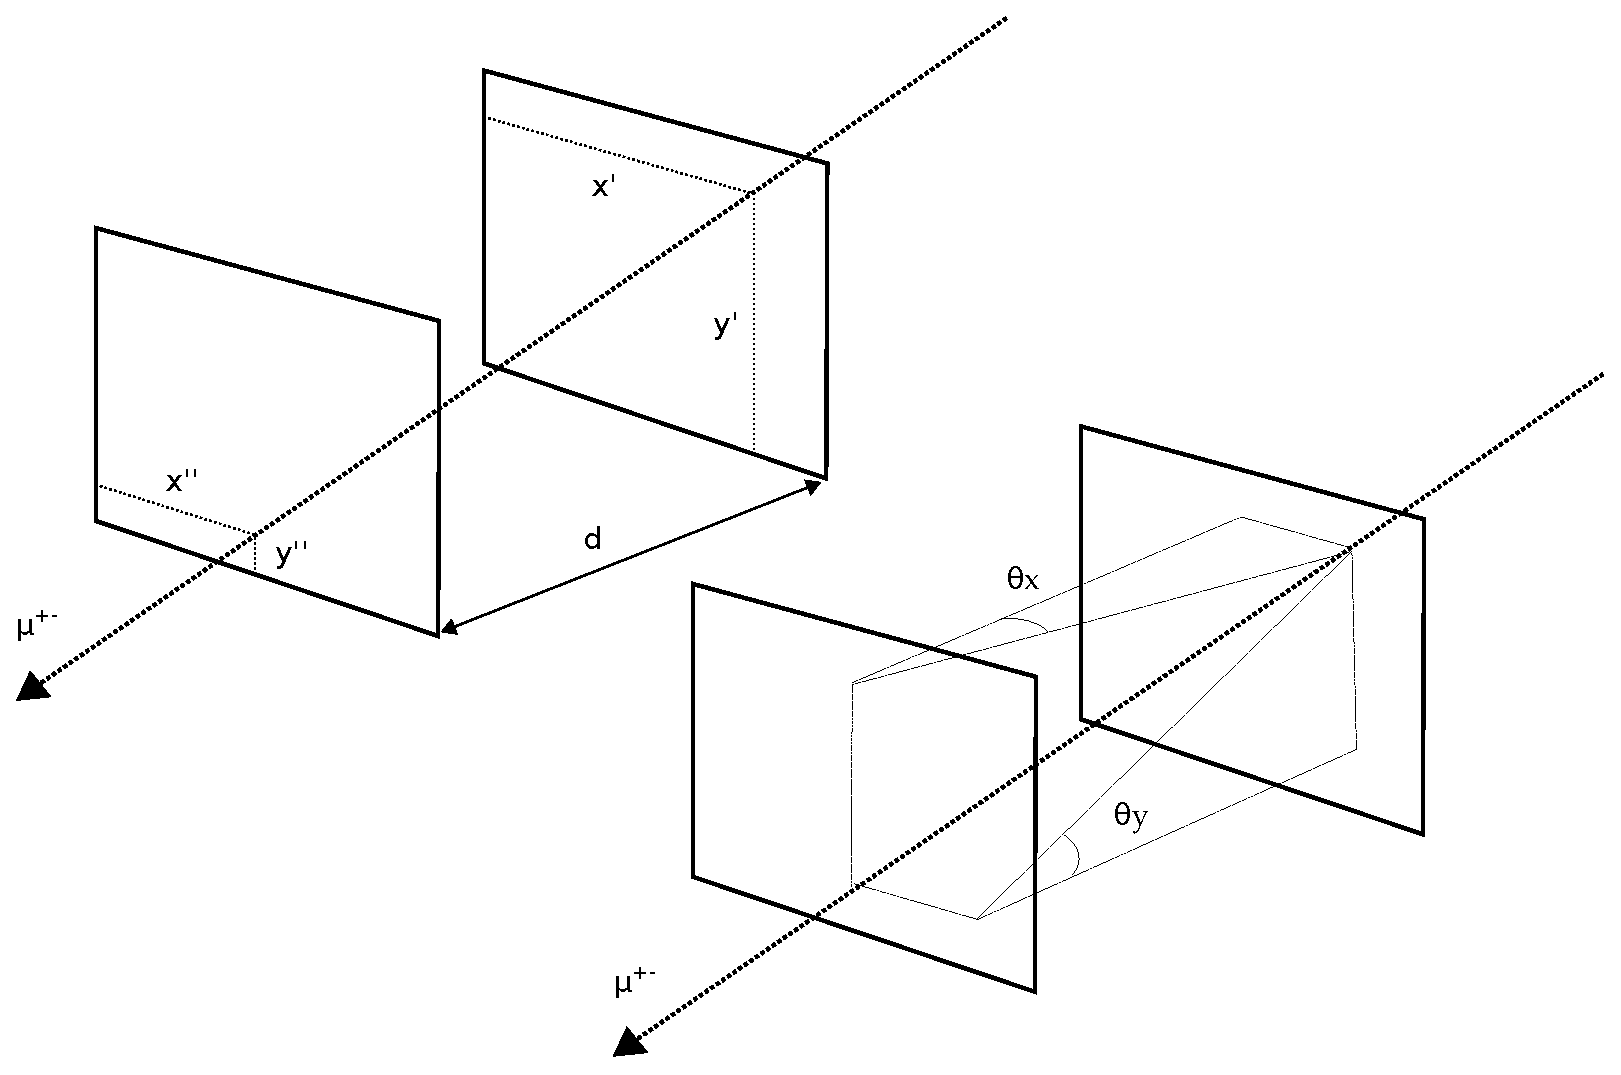
\includegraphics[width=0.8\textwidth]{Figures/Hodoscopio}
\caption[Principio de funcionamiento de un hodoscopio]{Principio de funcionamiento de un hodoscopio. El detector se conforma de al menos dos paneles, cada uno de los cuales mide la posición al paso de un muón $(x',y')$ por el panel frontal y $(x'',y'')$ por el panel trasero, luego se calcula su trayectoria en términos de los ángulos $\theta_x=\tan^{-1} (x^\prime - x^{\prime\prime})/d$ y $\theta_y=\tan^{-1} (y^\prime - y^{\prime\prime})/d$.}
\label{Hodoscopio}
\end{center}
\end{figure}

Finalmente, los paneles sensibles de un hodoscopio se basan en diferentes clases de detectores: centelladores segmentados \cite{Fujii2013, Lesparre2012, Tanaka2009}, centelladores contínuos \cite{Nagamine1995, Aguiar2015, Tang2016}, Cámaras de Plato Resistivo (RPC) \cite{Sehgal2016, Fehr2012}, Micromegas \cite{Bouteille2016}, Cámaras Proporcionales Multi-Hilo (MWPC) \cite{Olh2018} y láminas de emulsión \cite{Morishima2017, NAGAMINE2016}. Cada uno de éstos tiene ventajas y desventajas respecto a la resolución espacial, temporal, robustez mecánica, adquisición de la información y costo.\\

Los detectores anteriores se basan principalmente en tres técnicas de detección: centelladores plásticos (continuos y segmentados), emulsiones nucleares (láminas de emulsión) y detectores gaseosos (RPCs, MWPCs, Micromegas).

\subsection{Centelladores plásticos}

Los centelladores basan su principio de detección en el proceso de excitación y des-excitación de los electrones atómicos del material plástico cuando una partícula cargada lo atraviesa \cite{Grupen2008, Kleinknecht2005}.\\

Los fotones generados por la des-excitación son guiados, a través de una fibra óptica de corrimiento de longitud de onda (WLS), hasta el dispositivo sensor (tubo fotomultiplicador - PMT o fotomultiplicador de silicio - SiPM) como se ilustra en la Fig. \ref{Scintillator}. La fibra WLS tiene un desfase entre sus longitudes de onda de absorción y de emisión, lo cual le permite acoplar eficientemente el espectro de emisión del centellador y el espectro de absorción del elemento sensor. Ver la Fig. \ref{WLS}.

\begin{figure}[h!]
\begin{center}
\includegraphics[width=0.55\textwidth]{Figures/Scintillator}
\caption[Sistema de conexión típico entre un centellador segmentado, una fibra óptica WLS y un foto-sensor]{Sistema de conexión típico entre un centellador segmentado, una fibra óptica WLS y un foto-sensor \cite{Str2014}.}
\label{Scintillator}
\end{center}
\end{figure}

\begin{figure}[h!]
\begin{center}
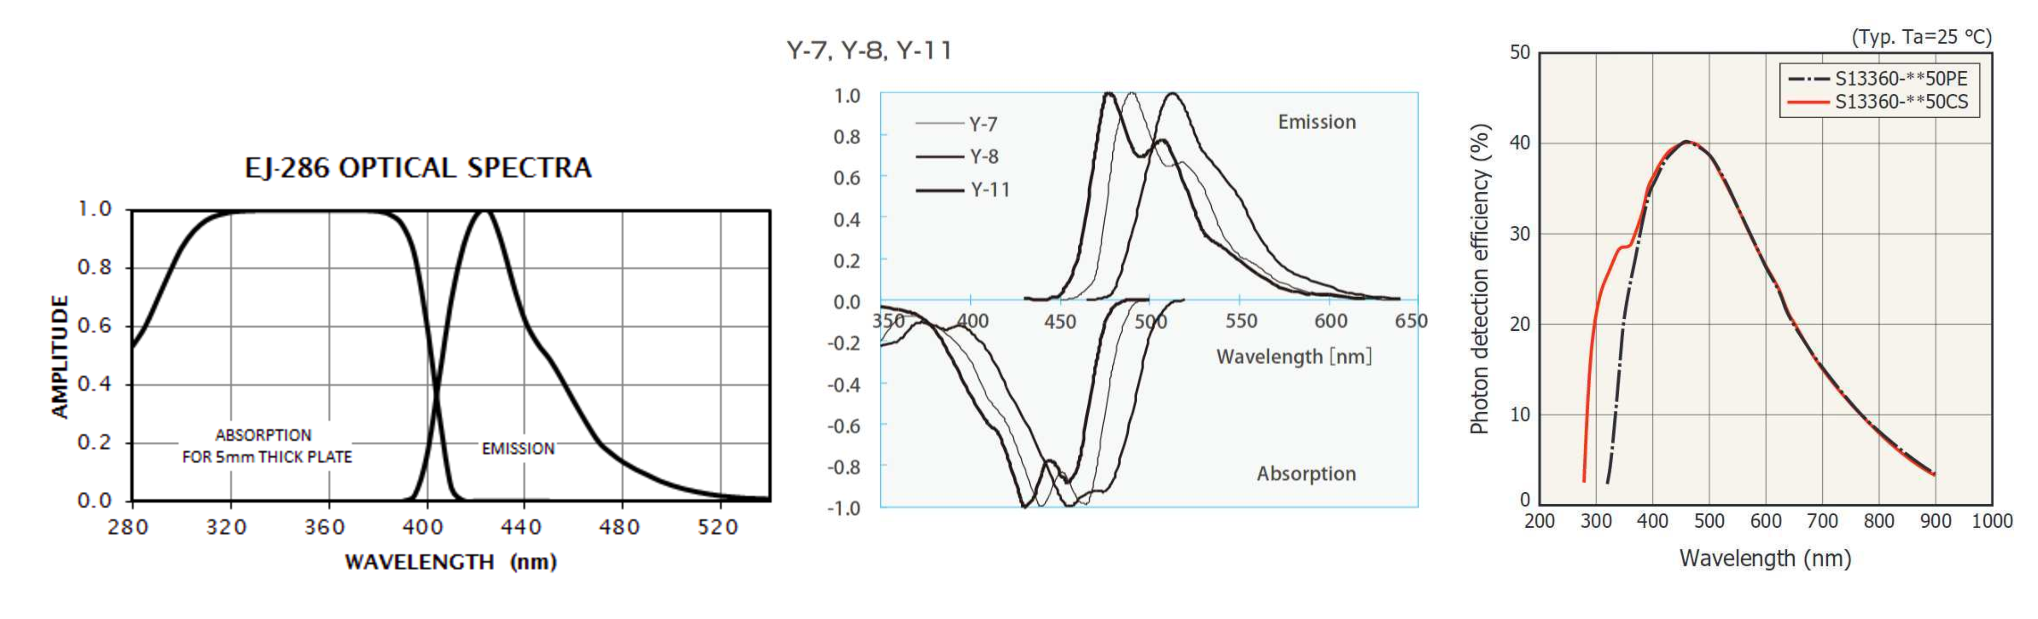
\includegraphics[width=1\textwidth]{Figures/WLS}
\caption[Espectros de absorción y emisión para una barra centelladora EJ-286 de ELJEN Technology, para tres WLS (Y-7, Y-8, Y-11) de Kurarayy el SiPM S13360-50CS de Hamamatsu ]{Espectros de absorción y emisión para una barra centelladora EJ-286 de ELJEN Technology \cite{Eljen2016}, para tres WLS (Y-7, Y-8, Y-11) de Kuraray \cite{Kuraray2018} y el SiPM S13360-50CS de Hamamatsu \cite{Hamamatsy2018}. El máximo de emisión del centellador es 430 nm y el de eficiencia del SiPM es 490 nm.}
\label{WLS}
\end{center}
\end{figure}

Los detectores de centelleo son robustos, fáciles de construir, relativamente económicos, insensibles a las condiciones ambientales y con una alta eficiencia de detección. Su principal desventaja es la resolución espacial. La cual es definida por la desviación estándar de una distribución uniforme, $w/\sqrt{12}$, donde $w$ es el ancho del centellador, \cite{Procureur2018}. 

\subsection{Emulsiones nucleares}

La técnica de emulsiones nucleares se basa en el principio de funcionamiento de la fotografía análoga. Cristales de haluro de plata son mezclados en una gelatina y revestidos sobre un sustrato de vidrio. La interacción de los haluros con los muones desencadena un proceso de oxido-reducción que los convierte en plata metálica \cite{Procureur2018}. Después de la exposición los haluros de plata restantes son disueltos dejando una cubierta negra sobre la posición de los muones, como se ve en la Fig. \ref{Emulsion} .  

\begin{figure}[h!]
\begin{center}
\includegraphics[width=0.45\textwidth]{Figures/Emulsion}
\caption[Imagen microscópica de la trayectoria de un muón (línea punteada) en una lámina de emulsión]{Imagen microscópica de la trayectoria de un muón (línea punteada) en una lámina de emulsión \cite{Nishiyama2014}.}
\label{Emulsion}
\end{center}
\end{figure}

Las láminas de emulsión tienen una alta resolución espacial ($\sim$ $\mu$m) y no consumen energía, sin embargo, el tiempo de vida de las láminas es corto ($\sim$ meses) y depende de la humedad y temperatura del ambiente en el cual se encuentre situado el detector. Adicionalmente, el análisis de datos es costoso debido al procesamiento de las imágenes obtenidas. Finalmente, con los datos registrados no se puede hacer un seguimiento temporal de los eventos, debido a que el proceso es acumulativo durante el tiempo de exposición.

\subsection{Detectores gaseosos}

Los detectores gaseosos tienen diferentes modos de trabajo según su tensión de polarización. En este caso el principio de funcionamiento del modo Geiger es: un gas ionizante es contenido entre dos capas de un material conductivo (ánodo y cátodo), un alto voltaje es aplicado entre los electrodos lo cual genera un campo eléctrico dentro del gas. Cuando una partícula cargada pasa a través del detector, esta interactúa con el gas generando pares ión-electrón. Los electrones son acelerados por efecto del campo eléctrico desprendiendo electrones secundarios del gas hasta causar un efecto avalancha como se muestra en la Fig. \ref{RPC}. Finalmente, los electrones son atraídos al ánodo generando una corriente eléctrica que es registrada posteriormente. 

\begin{figure}[h!]
\begin{center}
\includegraphics[width=0.6\textwidth]{Figures/Micromegas}
\caption[Principio de funcionamiento de un detector Micromegas]{Principio de funcionamiento de un detector Micromegas \cite{Procureur2018}. Los Micromegas se caracterizan por tener una rejilla interna cuya  función es amplificar la avalancha de electrones y, a su vez, acelerarla con el fin de disminuir el tiempo de respuesta del detector. En este caso, la rejilla genera un campo eléctrico de 40 kV/cm.}
\label{RPC}
\end{center}
\end{figure}

Este tipo de detectores poseen una alta resolución espacial ($\sim 0.1 mm$) a un costo razonable. Además, éstos permiten hacer una trazabilidad temporal de los eventos.\\

Sin embargo, los detectores gaseosos tienen varias desventajas. La ganancia depende altamente de variables ambientales como la presión y la temperatura. El alto voltaje de polarización necesario para su funcionamiento óptimo implica un riesgo latente de generación de chispas eléctricas que afectarían su integridad.  El gas ionizante debe fluir continuamente en el interior del detector con el fin de evitar el envejecimiento y degradación de los electrodos. Finalmente, las fugas de gas son inherentes e inevitables  elevando el costo del mantenimiento del detector.\\

En la Tabla \ref{tab1} se muestra una comparación de las principales características de los hodoscopios dependiendo de la tecnología de detección empleada.  \\

En este caso, los centelladores segmentados ofrecen la mejor alternativa de diseño debido a su bajo consumo energético, simplicidad y gran robustez mecánica, en comparación con las otras tecnologías. Todas estas ventajas se ven reflejadas en la disminución del tiempo de construcción del hodoscopio así como en la confiabilidad de su funcionamiento.\\

\begin{table}[ht]
\centering
  \caption{Comparación de las principales características de detección para hodoscopios basados en diferentes tecnologías.}
  \begin{tabular}{ | c | c | c |  c | c |  c | c |}
    \hline
   & \textbf{R. espacial} & \textbf{Voltaje} & \textbf{ToF}  & \textbf{Complejidad} & \textbf{Robustez**} & \textbf{Costo} \\ \hline
    \textbf{C. continuo*}   & baja  & $<$ 80 V &si  & baja  & alta  & bajo \\ \hline
    \textbf{C. segmentado*} & media & $<$ 80 V &si   & media & alta  & medio \\ \hline
    \textbf{RPCs}            & media & $>$ 8.5 kV &si   & alta  & baja &  alto \\ \hline
    \textbf{MWPCs}            & alta  & $>$ 1 kV &si   & alta  & media & alto \\ \hline
    \textbf{MicroMegas}      & alta  & $>$ 400 V &si   & alta  & media & alto \\ \hline
    \textbf{Emulsión}        & alta  & 0 & no   & baja  & baja  & bajo \\
    \hline
  \end{tabular}
  \label{tab1}
\end{table}

* Usando un fotomultiplicador de silicio (SiPM) como elemento sensor.\\
** Capacidad de un sistema para mantener un funcionamiento aceptable frente a situaciones imprevistas.\\


Finalmente, los hodoscopios utilizados para hacer muongrafía en estructuras volcánicas deben soportar diferentes condiciones meteorológicas, en el sitio de observación, sin ser afectados ni necesitar de un mantenimiento constante.

%####################### Fuentes Ruido ###########

\section{Fuentes de ruido en muongrafía}
La muongrafía es contaminada normalmente por tres fuentes de ruido: los muones de baja energía que son dispersados por la superficie de la estructura escaneada, los muones que ingresan por la parte posterior del detector (muones de albedo) y las partículas generadas por EAS entre el detector y el objeto estudiado.

\subsection{Dispersión de muones de baja energía}

La mayor parte del ruido que contamina la técnica de muongrafía ocurre por los muones de baja energía debido a la dispersión múltiple de Coulomb, \cite{Nishiyama2014,Gomez2017}. En este caso, la dirección del muón incidente en el detector no es la misma que su dirección original, Fig. \ref{Scattering}. La variación del ángulo de incidencia del muón $\Delta \theta = \theta_{fin}-\theta_{ini}$ ocurre por su interacción con los núcleos de los átomos que componen el objeto escaneado \cite{Furlan2013, Pesente2009}.

\begin{figure}[h!]
\begin{center}
\includegraphics[width=0.65\textwidth]{Figures/Muon_scattering.eps}
\caption[Dispersión de los muones incidentes de baja energía sobre la superficie]{Dispersión de los muones incidentes de baja energía sobre la superficie. El ángulo de incidencia del muón $\theta_{ini}$ varía debido a su interacción con el material que compone la estructura resultando en un ángulo dispersado $\theta_{fin}$. Adaptado de \cite{Gomez2017}.}
\label{Scattering}
\end{center}
\end{figure}


\begin{figure}[h!]
\begin{center}
\includegraphics[width=0.6\textwidth]{Figures/Scattering}
\caption[Variación angular, respecto a su dirección de incidencia, de los muones atmosféricos después de atravesar 10 m, 100 m y 1000 m de roca estándar]{Variación angular, respecto a su dirección de incidencia, de los muones atmosféricos después de atravesar 10 m, 100 m y 1000 m de roca estándar. La línea roja representa el umbral de energía mínima sobre el cual los muones logran emerger del medio sin ser absorbidos.}
\label{Scattering_Variance}
\end{center}
\end{figure}

Para evaluar los efectos de la dispersión en los muones incidentes se debe tener en cuenta la energía mínima requerida para atravesar el material, tal como se puede apreciar en la  Fig. \ref{Scattering_Variance}.\\

La dispersión múltiple de Coulomb se puede representar como una distribución Gausiana con media cero y con una desviación estándar $\sigma_\theta$ que depende de la longitud de radiación $X_0$, del espesor del material $x$, de la cantidad de movimiento $p$ y velocidad $\beta$ del muón  \cite{Grupen2008}:

\begin{equation}
\sigma_\theta \approx \frac{13.6 \text{MeV}}{\beta p c} \sqrt{\frac{x}{X_0}}
\end{equation}

\begin{equation}
X_0 = \frac{716.4 (\text{g/cm}^2)}{\rho} \frac{A}{Z(Z+1)\ln (287/\sqrt{Z})}
\end{equation}
donde $\rho$ es la densidad y $Z$ es el número atómico efectivo del material atravesado.


\subsection{Muones de albedo}

Otro factor que repercute en la contaminación de la muongrafía son los muones cuasi-horizontales ($\theta >= 75^{\circ}$) que inciden en el detector desde la parte posterior. El momento promedio de los también llamados muones de albedo es de $\approx 10 GeV/c$ \cite{Nishiyama2014}. Estas partículas trazan trayectorias similares a los muones emergentes desde el volcán generando eventos de coincidencia en el detector. Ver Fig. \ref{Albedo}.

\begin{figure}[h!]
\begin{center}
\includegraphics[width=0.65\textwidth]{Figures/Albedo.eps}
\caption[Detección de un evento falso debido a un muón que incide por la parte posterior del detector]{Detección de un evento falso debido a un muón que incide por la parte posterior del detector. La partícula atraviesa el hodoscopio emulando una trayectoria válida proveniente desde la estructura escaneada con un ángulo 180$^\circ$ - $\theta_{ini}$.}
\label{Albedo}
\end{center}
\end{figure}

El espectro de muones a nivel del mar $\Phi(p,\theta,h=0m)$ como función del momento $p$ y el ángulo cenital $\theta$ es dado por \cite{Reyna2006}:


\begin{align*}
\Phi(p,\theta,0) &= \cos^3\theta\Phi_V(p \cos \theta),\\
\Phi_V(\zeta) &= c_1 \zeta^{-(c_2+c_3\log_{10}\zeta+c_4(\log_{10}\zeta)^2+c_5(\log_{10}\zeta)^3)},\\
c_1 &= \text{0.00253cm}^{-2}s^{-1}sr^{-1}(GeV/c^{-1}),\\
c_2 &= \text{0.2455},c_3=\text{1.288},c_4=\text{-0.2555},c_5=\text{0.0209}
\end{align*}

donde $\zeta=p\cos\theta$.

\begin{figure}[h!]
\begin{center}
\includegraphics[width=0.65\textwidth]{Figures/Muon_spectrum.png}
\caption[Espectro de energía de muones atmosféricos a diferentes ángulos cenitales]{Espectro de energía de muones atmosféricos a diferentes ángulos cenitales \cite{Ariga2018, Vesga2018, Valencia2016}. El flujo diferencial de muones disminuye a medida que aumenta el ángulo cenital, teniendo una atenuación hasta de dos órdenes de magnitud a 75$^\circ$ (violeta) en comparación con el flujo a 0$^\circ$ (rojo).}
\label{Muon_spectrum}
\end{center}
\end{figure}

Como se puede ver en la Fig. \ref{Muon_spectrum} el flujo de muones a nivel del mar disminuye a medida que el ángulo cenital aumenta. Por otro lado, el momento promedio aumenta con el incremento del cenit teniendo de esta manera que el momento promedio para los muones verticales es de $\approx$ 4 GeV/c y de los quasi-horizontales es de $\approx$ 10 GeV/c.\\

Esta fuente de ruido puede ser significativa si el detector se encuentra ubicado en un sitio en el cual no tenga ninguna clase de protección en su parte posterior, por ejemplo, cadenas montañosas que sirvan como filtro a estos muones quasi-horizontales.

\subsection{Componente electromagnética (EM) de EAS}

La tercera fuente de contaminación en la muongrafía ocurre debido a partículas secundarias (PS) generadas por EAS entre la estructura escaneada y el detector. Ver Fig. \ref{EAS}.\\

Las PS están compuestas principalmente por $p,n,\mu^{\pm},\pi^{\pm},e^{\pm}$ y $\gamma$. El flujo de PS como función de la energía cinética es presentado en la Fig. \ref{Particle_Flux}. El flujo de PS a nivel del mar es estimado, por medio de una simulación, teniendo en cuenta el espectro de rayos cósmicos primarios que inciden sobre la atmósfera terrestre. En la simulación la componente  electromagnética es cortada bajo 1 MeV para $e^{\pm}$ y bajo 100 keV para $\gamma$.

\begin{figure}[h!]
\begin{center}
\includegraphics[width=0.65\textwidth]{Figures/EAS.eps}
\caption[Detección de un evento falso debido a la incidencia de un $e^-$ generado en una EAS entre el objeto escaneado y el detector]{Detección de un evento falso debido a la incidencia de un $e^-$ generado en una EAS entre el objeto escaneado y el detector. Las partículas cargadas de la componente EM de las EAS generan un aumento en el flujo estimado al atravesar el hodoscopio.}
\label{EAS}
\end{center}
\end{figure}

Las partículas más abundantes son los $\gamma$ seguidos por los $n$ y $\mu^{\pm}$. Los $e^{\pm}$ y $p$ tienen flujos menores y los $\pi^{\pm}$ son tres órdenes de magnitud menos probables.\\

\begin{figure}[h!]
\begin{center}
\includegraphics[width=1\textwidth]{Figures/PS_Flux}
\caption[Flujo de PS simulado a nivel del volcán Cerro Machín]{Flujo de PS simulado a nivel del volcán Cerro Machín para el Telescopio de Muones (MuTe) en Colombia, \cite{Vasquez2018, Valencia2016}. El espectro esta compuesto por los flujos individuales de $p,n,\mu^{\pm},\pi^{\pm},e^{\pm}$ y $\gamma$. En este caso, predominan dos jorobas, una centrada en $\sim 10$ MeV/c compuesta por $e^{\pm}$ y $\gamma$ y otra a $\sim 3$ GeV/c compuesta por $\mu^{\pm}$.}
\label{Particle_Flux}
\end{center}
\end{figure}

La estructura general del espectro de PS a nivel de suelo tiene dos jorobas predominantes que se solapan alrededor de 0.3 GeV/c. La primera joroba representa la componente electromagnética de la EAS y está compuesta principalmente por $e^{\pm}$ y $\gamma$. Por otro lado, la segunda joroba representa la componente muónica conformada por $\mu^{\pm}$.\\

Las PS generan eventos falsos de dos maneras:

\begin{itemize}
    \item Mediante la coincidencia accidental de dos o más partículas incidentes en el detector lo cual mimetiza una trayectoria generada por un muón \cite{KUSAGAYA2015}.
    \item Una partícula individual con energía suficiente para atravesar todo el detector.
\end{itemize}

Teniendo en cuenta que la muongrafía hace una estimación de la distribución densidad interna de la estructura dependiendo del flujo diferencial de los muones que la atraviesan, un aumento en el flujo registrado debido a los eventos falsos repercute en una sub-estimación de la densidad de la estructura, \cite{Nishiyama2014}.

%############# Eliminación de Ruido #######################

\section{Eliminación de ruido en muongrafía}

La discriminación de eventos falsos en muongrafía presenta un reto actual. Este proceso se puede efectuar mediante la medición de las características diferenciadoras entre las partículas que generan señal y las que generan ruido.\\

En este contexto, las técnicas de identificación de partículas (PID) surgen como solución en la tarea de discriminación \cite{Nishiyama2016}. Las técnicas PID se basan principalmente en la medición de 4 variables: el tiempo de vuelo (ToF), la pérdida de energía, la radiación Cherenkov (contadores, RICH y DISC) y la radiación de transición. En la Fig. \ref{PID} se muestra una comparación de los métodos PID y su rango de operación.

\begin{figure}[h!]
\begin{center}
\includegraphics[width=0.8\textwidth]{Figures/PID}
\caption[]{Comparación de métodos PID para diferenciar $\pi^{\pm}$ y $K^{\pm}$ \cite{Kleinknecht2005}}
\label{PID}
\end{center}
\end{figure}

Las principales componentes del ruido de fondo en muografía son muones y electrones de baja energía ($<$ 1 GeV), por lo cual pueden ser identificadas mediante la medición de la pérdida de energía, los contadores Cherenkov o sistemas ToF.

\subsection{Medición del tiempo de vuelo}

La medición del ToF de la partícula permite estimar su velocidad, su momento \cite{Best2015} y su identidad \cite{Gruttola2014, Kolanoski2016}. Adicionalmente, la medición del momento en muongrafía puede ser usada para filtrar las partículas con momento $<$ 1 GeV/c las cuales componen la principal fuente de ruido en esta técnica como se reporta en \cite{Nishiyama2014,Gomez2017}.

En la Fig. \ref{ToF} (línea sólida) se muestra el ToF  para muones con momento entre 0.1 GeV/c y 100 GeV/c medido por un hodoscopio de dos paneles centelladores con una separación de 1 m. A medida que el cantidad de movimiento aumenta el ToF decrece hasta que llega a una zona de saturación debido a los límites relativistas para momentos $>$ 1 GeV/c, en esta región el ToF es $\approx 3.3 ns$.

\begin{figure}[h!]
\begin{center}
\includegraphics[width=0.55\textwidth]{Figures/ToF_Mix.png}
\caption[Resolución del ToF necesaria para diferenciar muones con momento entre 0.1 GeV/c y 100 GeV/c con un $\sigma_p = 10$ MeV]{(Línea sólida): Tiempo de vuelo para muones con momento entre 0.1 GeV/c y 100 GeV/c al atravesar un hodoscopio de dos paneles con 1 m de separación \cite{Williams2012, Best2015}. (Línea punteada): Resolución del ToF necesaria para diferenciar muones con momento entre 0.1 GeV/c y 100 GeV/c con un $\sigma_p = 10$ MeV al atravesar un hodoscopio de dos paneles con 1 m de separación \cite{Genat2009, Lippmann2012}.}
\label{ToF}
\end{center}
\end{figure}

% \begin{figure}[h!]
% \begin{center}
% \includegraphics[width=0.55\textwidth]{Figures/ToF_Resolution.png}
% \caption[Resolución del ToF necesaria para diferenciar muones con momento entre 0.1 GeV/c y 100 GeV/c con un $\sigma_p = 10$ MeV]{Resolución del ToF necesaria para diferenciar muones con momento entre 0.1 GeV/c y 100 GeV/c con un $\sigma_p = 10$ MeV al atravesar un hodoscopio de dos paneles con 1 m de separación \cite{Genat2009, Lippmann2012}.}
% \label{Resolution}
% \end{center}
% \end{figure}

La resolución del momentum del detector mide su habilidad para distinguir partículas con momentos cercanos. En este caso, la resolución de la cantidad de movimiento depende de la resolución del ToF. Para el hodoscopio anteriormente expuesto la resolución del ToF para muones con momentos entre de 0.1 GeV/c y 100 GeV/c se expone en la Fig. \ref{ToF} (línea punteada). Por ejemplo, para medir un momento de 1 GeV/c con una $\sigma_p = 10$ MeV es necesario un $\delta_{ToF}\approx$ 1 ps y para 10 GeV/c un $\delta_{ToF}\approx$ 0.003 ps.\\

%Adicionalmente, el ToF es también usado para identificación de partículas \cite{Kolanoski2016}. En este caso, ofrecería una herramienta para diferenciar los $e^{\pm}$ provenientes de EAS de los $\mu^{\pm}$ emergentes desde el volcán.\\

En la Fig. \ref{ToF_mue} se muestra el ToF registrado en un hodoscopio, con 1 m de separación entre sus planos, para $\mu^{\pm}$ y $e^{\pm}$ a nivel del mar teniendo en cuenta su espectro de la Fig. \ref{Particle_Flux}. En este caso, el proceso de discriminación es viable para momentos $\le 10$ MeV/c para $e^{\pm}$ y $\le 2$ GeV/c para $\mu^{\pm}$ , por encima de estos valores estas partículas describen el mismo ToF. \\

El ToF permite además discriminar los muones de albedo debido a que muestran un ToF negativo ya que inciden primero en el panel posterior del hodoscopio.

\begin{figure}[h!]
\begin{center}
\includegraphics[width=0.5\textwidth]{Figures/ToF_Spec.png}
\caption{Tiempo de vuelo para $\mu^{\pm}$ (verde) y $e^{\pm}$ (rojo) al atravesar un hodoscopio de dos paneles con 1 m de separación. El límite de discriminación de $\mu^{\pm}$ es $\sim$ 2 GeV y para $e^{\pm}$ de $\sim$ 10 MeV}
\label{ToF_mue}
\end{center}
\end{figure}
 
\subsection{Medición de la pérdida de energía}

La estimación de la -dE/dx se hace por medio de un calorímetro el cual puede ser continuo o segmentado. Este dispositivo mide la cantidad de luz generada por la partícula incidente al ionizar el medio que cruza.\\

Los contadores Cherenkov miden los fotones generados por una partícula cargada al cruzarlo. En este caso, cuando la velocidad de la partícula es mayor a la velocidad de la luz en el medio, el medio sufre un proceso de polarización-depolarización que genera una onda electromagnética plana por interferencia constructiva \cite{Kolanoski2016}.\\

El ángulo de emisión de los fotones Cherenkov $\theta_c$ es definido como:

\begin{equation}
    \cos \theta_c = \frac{1}{n\beta}
\end{equation}
donde $n$ es el índice de refracción del medio.

\begin{figure}[h!]
\begin{center}
\includegraphics[width=0.5\textwidth]{Figures/dNdx_spec.png}
\caption[Fotones Cherenkov por unidad de longitud generados por $\mu^{\pm}$ y $e^{\pm}$ a nivel del mar en el rango de 300nm $< \lambda <$ 570nm]{Fotones Cherenkov por unidad de longitud generados por $\mu^{\pm}$ y $e^{\pm}$ a nivel del mar en el rango de 300nm $< \lambda <$ 570nm\cite{Vasquez2018, Motta2018}.}
\label{dNdx}
\end{center}
\end{figure}

Así mismo, el número de fotones Cherenkov por unidad de longitud es:

\begin{equation}
   \frac{dN}{dx}=2 \pi \alpha z^2 \int_{\lambda_1}^{\lambda_2} \left(1- \frac{1}{n^2 \lambda \beta^2} \right) \frac{d \lambda}{\lambda^2} \approx 2 \pi \alpha z^2 \sin^2 \theta_c \left( \frac{\lambda_2-\lambda_1}{\lambda_2 \lambda_1} \right) 
\end{equation}

donde $\alpha$ es la constante de estructura fina, $z$ representa la carga de la partícula en unidades de la carga del electrón $e$ y $\lambda$ es la longitud de onda de la radiación Cherenkov.\\ 

Por ejemplo, para un rango de longitudes de onda que incluye el espectro visible y ultravioleta ($\lambda_1 =$ 300 nm - $\lambda_2 =$ 570 nm) tenemos:

\begin{equation}
   \frac{dN}{dx} \approx 723 \sin^2 \theta_c \ \text{[photons/cm]}
\end{equation}

%La medición de la pérdida de energía (-dE/dx) permite la identificación de partículas \cite{Klinger2015}.

En la Fig. \ref{dNdx} se muestra el número de fotones Cherenkov (dN/dx) por centímetro que generan los $e^{\pm}$ y $\mu^{\pm}$ en un contador Cherenkov de agua. En este caso, la dN/dx para $e^{\pm} > $  10 MeV/c y para $\mu^{\pm} > $ 2 GeV/c es de $\approx 315$ fotones/cm. 

\begin{figure}[h!]
\begin{center}
\includegraphics[width=1\textwidth]{Figures/e_mu_hist.png}
\caption[Histograma del número total de fotones Cherenkov generados por $1\times10^5$ $e^-$ de 20 MeV y $1\times10^5$ $\mu^-$ de 3 GeV en un contador Cherenkov de agua]{Histograma del número total de fotones Cherenkov generados por $1\times10^5$ $e^-$ de 20 MeV y $1\times10^5$ $\mu^-$ de 3 GeV en un contador Cherenkov de agua \cite{Vasquez2018}.}
\label{N_mue}
\end{center}
\end{figure}

No obstante, los $e^{\pm}$ son frenados rápidamente por el medio debido a su pérdida de energía generando un número total de fotones $N$ menor al causado por los $\mu^{\pm}$ los cuales recorren una distancia mayor. En la Fig. \ref{N_mue} se muestran los histogramas del número de fotones que alcanzan el dispositivo sensor (PMT) en un detector Cherenkov cúbico de agua con 1.2 m de lado. \\

Debido a que los $e^{\pm}$ pueden recorrer una longitud promedio de 10 cm siendo $N \approx 200$, en contraste, los $\mu^{\pm}$ atraviesan totalmente el contador Cherenkov generando $N \approx 1600$. Teniendo en cuenta esto, la medición de la radiación Cherenkov permite separar la componente electromagnética y la componente muónica de las EAS.

\input{Methodology/Methodology.tex}
%\input{Plan/Plan}
\input{Schedule/Schedule.tex}
\input{Founding/Founding.tex}

%\input{Actual/Actual}
%\input{Conclusions/Conclusions}

\newpage
%%%%%%%%%%%%%%%%%%%%%%%%% Bibliografia %%%%%%%%%%%%%%%%%%%%%5
\cleardoublepage
\addcontentsline{toc}{chapter}{Bibliografía}%para que aparezca en la tabla de contenidos
\bibliographystyle{unsrt}
\bibliography{Bibliography/MuTe.bib}
%Archivo con las referencias bibliográficas, creado en JabRef (o manualmente)

\end{document}
